% Содержимое отчета по курсу Анализ алгоритмов

\aaunnumberedsection{ВВЕДЕНИЕ}{sec:intro}

\textbf{Параллелизм} описывает одновременное выполнение различных последовательностей действий~\cite{posix-threads}. Следовательно, параллельные вычисления подразумевают выполнение операций одновременно. Распараллеливание вычислений может повысить временную эффективность программы на многопроцессорных системах и даже на однопроцессорных, если программа часто простаивает, ожидая ввода-вывода~\cite{tanenbaum}.

В современных системах параллельность может быть реализована с использованием потоков или процессов. При этом важно учитывать, что программы часто работают не в строгом параллелизме, а конкурентно, выполняясь последовательно с частым переключением между задачами~\cite{tanenbaum}.

Цель данной работы — разработка программного обеспечения для скачивания страниц с сайта vkusnoprigotovim.ru.

Задачи работы включают:

\begin{itemize}
	\item создание ПО для однопоточного скачивания и парсинга;
	\item создание многопоточного ПО для скачивания и парсинга;
	\item исследование временных характеристик разработанных программ.
\end{itemize}

\aasection{Входные и выходные данные}{sec:input-output}

Входными данными для программы является адрес главной страницы ресурса vkusnoprigotovim.ru.
Выходными данными является директория с файлами, которые содержат скачанные данные со страниц в текстовом формате.

\aasection{Преобразование входных данных в выходные}{sec:algorithm}

Для реализации ПО был использован язык C\#, поддерживающий нативную многопоточность. Класс System.Threading.Thread представляет собой абстракцию над системными потоками, позволяющую вызывать их из кода программы~\cite{nutshell}. Вызов метода Thread.Start влечет за собой создание системного потока, отдельного от основного потока программы~\cite{Thread.Start}.
 
\textbf{Алгоритм обработки набора страниц}

\begin{enumerate}
    \item Инициализация начальных параметров: начальный URL, директория для сохранения страниц, максимальное количество страниц и путь для сохранения результатов в формате CSV.
    \item Определение количества потоков для тестирования и числа повторений тестов.
    \item Открытие CSV-файла для записи результатов и добавление заголовка.
    \item Проведение тестов в последовательном режиме:
    \begin{itemize}
        \item запуск цикла тестирования на заданное количество повторений;
        \item инициализация объекта \texttt{WebScraper} с настройками для последовательного режима;
        \item измерение времени выполнения операции с помощью \texttt{Stopwatch};
        \item сохранение времени выполнения теста.
    \end{itemize}
    \item Запись среднего времени выполнения последовательного режима в CSV и вывод в консоль.
    \item Проведение тестов в параллельном режиме с использованием различных значений количества потоков:
    \begin{itemize}
        \item запуск цикла по каждому значению количества потоков;
        \item инициализация объекта \texttt{WebScraper} с настройками для параллельного режима;
        \item измерение времени выполнения операций для каждого количества потоков;
        \item сохранение времени выполнения теста.
    \end{itemize}
    \item Запись среднего времени выполнения параллельного режима для каждого количества потоков в CSV и вывод в консоль.
    \item Завершение тестирования и закрытие CSV-файла.
    \item Вывод сообщения о завершении работы и сохранении результатов.
\end{enumerate}

\textbf{Ниже представлено описание работы класса \texttt{WebScraper}.}
\begin{enumerate}
    \item Инициализация объекта \texttt{WebScraper} с базовым URL, максимальным количеством страниц, директорией для сохранения и количеством потоков.
    \item Создание очереди URL и списка для отслеживания обработанных URL.
    \item Начало работы скрапинга с проверкой на параллельный режим:
    \begin{itemize}
        \item в параллельном режиме инициализация и запуск нескольких потоков, каждый из которых выполняет метод \texttt{ProcessQueueParallel};
        \item в последовательном режиме выполнение метода \texttt{ProcessQueueSequential}.
    \end{itemize}
    \item Обработка страниц в последовательном режиме, извлечение URL из очереди и вызов метода \texttt{ProcessPage}.
    \item Обработка страниц в параллельном режиме:
    \begin{itemize}
        \item попытка извлечь URL из очереди с помощью семафора;
        \item вызов метода \texttt{ProcessPage} для обработки страницы.
    \end{itemize}
    \item Метод \texttt{ProcessPage}:
    \begin{itemize}
        \item проверка URL на соответствие базовому домену и уникальность;
        \item запрос страницы и извлечение текста с нужными классами с помощью метода \texttt{ExtractTextFromBody};
        \item сохранение содержимого страницы в текстовый файл;
        \item извлечение ссылок со страницы и добавление их в очередь, если они еще не обработаны.
    \end{itemize}
    \item Метод \texttt{ExtractTextFromBody} фильтрует текст HTML-страницы по классам и форматирует его.
    \item Метод \texttt{ExtractLinks} извлекает и фильтрует ссылки, соответствующие базовому домену.
\end{enumerate}

\aasection{Примеры работы программы}{sec:demo}

Один из примеров обработки веб-страниц~\cite{receipt} представлен на рисунках~\ref{before}--\ref{after}.

\begin{figure}[H]
	\centering
	
\includegraphics[width=0.9\textwidth]{img/before.png}
	\caption{Веб-страница по ссылке~\cite{receipt}}
	\label{before}
\end{figure}

\begin{figure}[H]
	\centering
	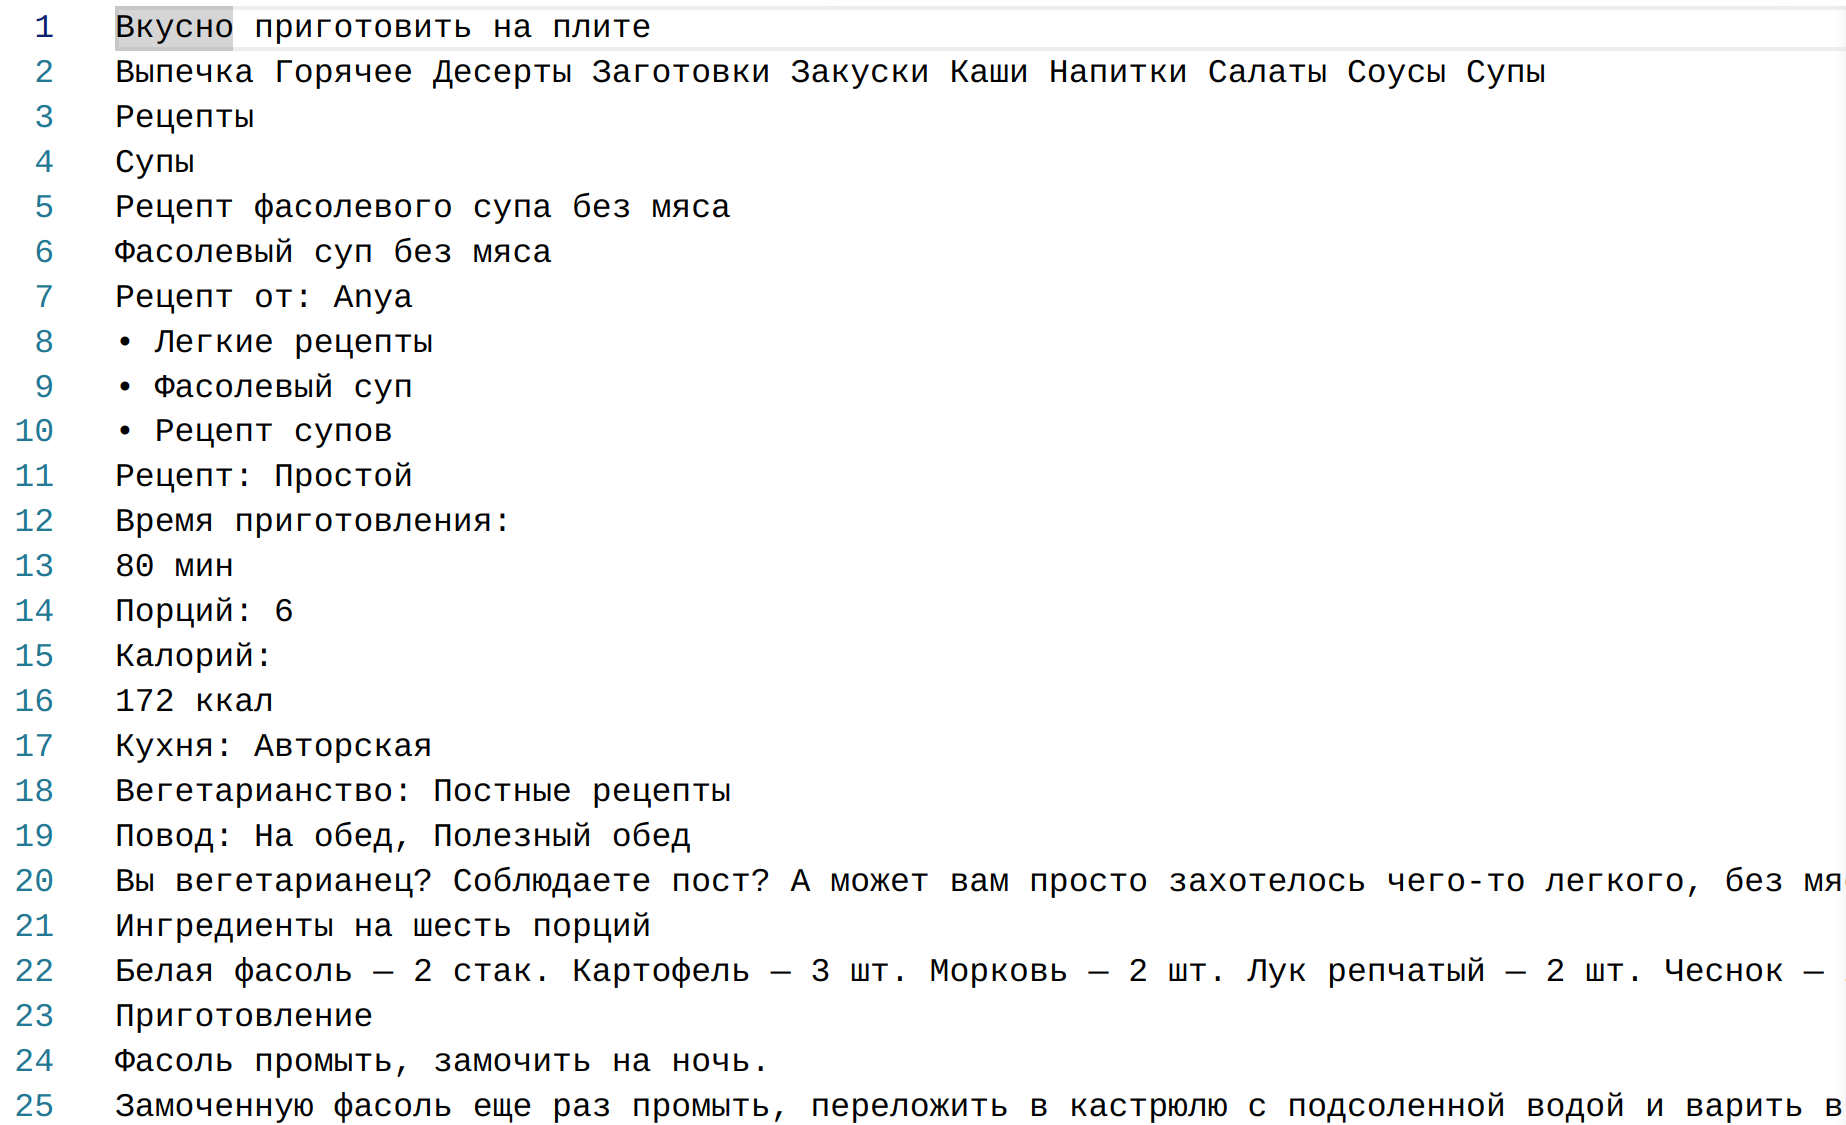
\includegraphics[width=0.9\textwidth]{img/after.png}
	\caption{Результат обработки программой}
	\label{after}
\end{figure}

\aasection{Тестирование}{sec:tests}

Тестирование программы проводилось загрузкой в качестве входных данных 100 ссылок на различные страницы vkusnoprigotovim.ru. При этом отслеживалось количество удачных скачиваний и обработок страницы, а также выборочная ручная проверка 10 случайных выходных файлов. 

Тестирование проводилось как для однопоточной реализации, так и для многопоточной, при этом выходные файлы обоих реализаций при тестировании оказались идентичными.

Тестирование было успешно пройдено.

\aasection{Описание исследования}{sec:study}

В ходе исследования были собраны данные о временных характеристиках однопоточной и многопоточной реализаций, при этом для многопоточной реализации были собраны данные при количестве потоков равному 1, 2, 4, 8, 16, 32, 64.

Для каждого из вариантов программы выполнение проводилось 10 раз и бралось среднее арифметическое времён, на вход подавался файл с 100 ссылок.

Технические характеристики устройства,на котором проводились замеры:

\begin{itemize}
	\item процессор: AMD Ryzen 7 5800U (16) @ 4.51 ГГц;
	\item ооеративная память: 16 Гб;
	\item ядро ОС Linux 6.11.6-zen1-1-zen.
\end{itemize}

При проведении замеров ноутбук был включён в сеть и были запущены только системные приложения.

Временные характеристики реализаций представлены в таблице~\ref{tbl:time} и на графике~\ref{plot}.

\begin{figure}[h]
	\centering
	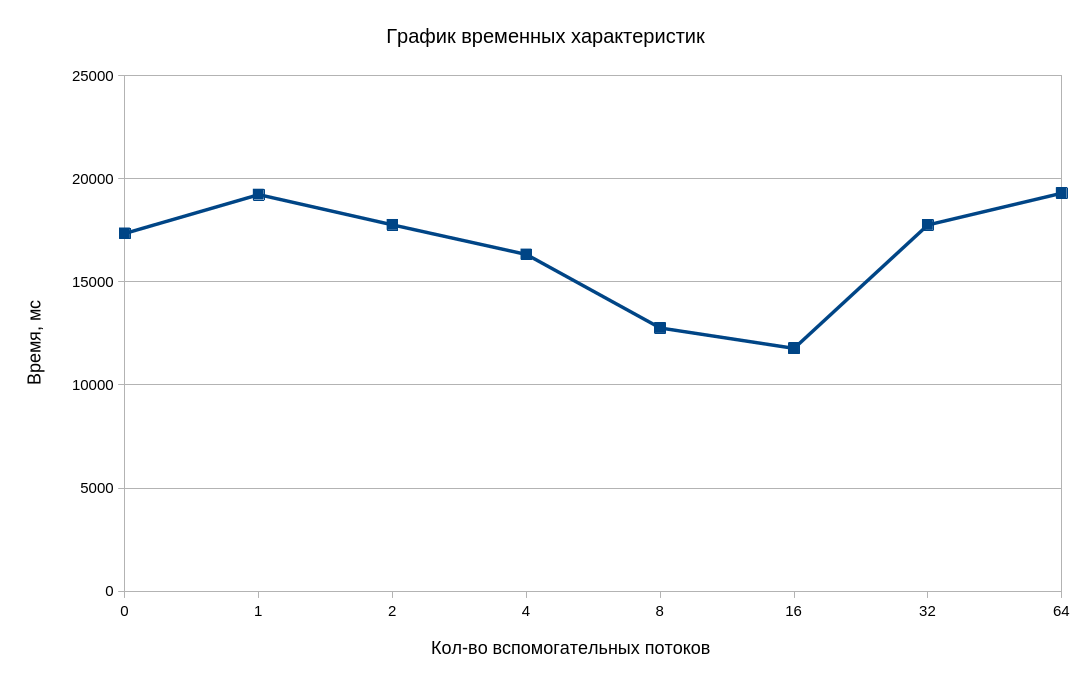
\includegraphics[width=\textwidth]{img/graph.png}
	\caption{График временных характеристик разработанных программ}
	\label{plot}
\end{figure}

\begin{longtable}{|c|r|}
    \caption{Временные характеристики разработанных программ (начало)}\label{tbl:time}
    \\
    \hline
    Кол-во вспомогательных потоков & Время, мс \\
    \hline
    \endfirsthead
    \caption{Временные характеристики разработанных программ (окончание)}
    \\
    \hline
    Кол-во вспомогательных потоков & Время, мс     \\
    \hline
    \endhead
    \hline
    \endfoot
    \endlastfoot
    \hline
    0 &	17346     \\ \hline
    1 &	19227     \\ \hline
    2 &	17761     \\ \hline
    4 &	16326     \\ \hline
    8 &	12763     \\ \hline
    16 &	11771     \\ \hline
    32 &	17758     \\ \hline
    64 &	19297     \\ \hline
\end{longtable}

\aaunnumberedsection{ЗАКЛЮЧЕНИЕ}{sec:outro}

Было разработано программное обеспечение для скачивания страниц с сайта vkusnoprigotovim.ru.

В ходе работы были решены следующие задачи:
\begin{itemize}
	\item разработано ПО, выполняющее скачивание и парсинг в одном потоке;
	\item разработано многопоточное ПО, выполняющее скачивание и парсинг;
	\item исследованы временные характеристики разработанных программ.
\end{itemize}

В ходе исследования было выявлено, что использование параллельных вычислений на нативных потоках ускоряет программу, однако использование большего числа потоков, чем может выполнять процессор не даёт прироста производительности, а замедляет программу.